\documentclass{article}\usepackage[]{graphicx}\usepackage[]{xcolor}
% maxwidth is the original width if it is less than linewidth
% otherwise use linewidth (to make sure the graphics do not exceed the margin)
\makeatletter
\def\maxwidth{ %
  \ifdim\Gin@nat@width>\linewidth
    \linewidth
  \else
    \Gin@nat@width
  \fi
}
\makeatother

\definecolor{fgcolor}{rgb}{0.345, 0.345, 0.345}
\newcommand{\hlnum}[1]{\textcolor[rgb]{0.686,0.059,0.569}{#1}}%
\newcommand{\hlsng}[1]{\textcolor[rgb]{0.192,0.494,0.8}{#1}}%
\newcommand{\hlcom}[1]{\textcolor[rgb]{0.678,0.584,0.686}{\textit{#1}}}%
\newcommand{\hlopt}[1]{\textcolor[rgb]{0,0,0}{#1}}%
\newcommand{\hldef}[1]{\textcolor[rgb]{0.345,0.345,0.345}{#1}}%
\newcommand{\hlkwa}[1]{\textcolor[rgb]{0.161,0.373,0.58}{\textbf{#1}}}%
\newcommand{\hlkwb}[1]{\textcolor[rgb]{0.69,0.353,0.396}{#1}}%
\newcommand{\hlkwc}[1]{\textcolor[rgb]{0.333,0.667,0.333}{#1}}%
\newcommand{\hlkwd}[1]{\textcolor[rgb]{0.737,0.353,0.396}{\textbf{#1}}}%
\let\hlipl\hlkwb

\usepackage{framed}
\makeatletter
\newenvironment{kframe}{%
 \def\at@end@of@kframe{}%
 \ifinner\ifhmode%
  \def\at@end@of@kframe{\end{minipage}}%
  \begin{minipage}{\columnwidth}%
 \fi\fi%
 \def\FrameCommand##1{\hskip\@totalleftmargin \hskip-\fboxsep
 \colorbox{shadecolor}{##1}\hskip-\fboxsep
     % There is no \\@totalrightmargin, so:
     \hskip-\linewidth \hskip-\@totalleftmargin \hskip\columnwidth}%
 \MakeFramed {\advance\hsize-\width
   \@totalleftmargin\z@ \linewidth\hsize
   \@setminipage}}%
 {\par\unskip\endMakeFramed%
 \at@end@of@kframe}
\makeatother

\definecolor{shadecolor}{rgb}{.97, .97, .97}
\definecolor{messagecolor}{rgb}{0, 0, 0}
\definecolor{warningcolor}{rgb}{1, 0, 1}
\definecolor{errorcolor}{rgb}{1, 0, 0}
\newenvironment{knitrout}{}{} % an empty environment to be redefined in TeX

\usepackage{alltt}
\usepackage{hyperref}
\usepackage[margin=1in]{geometry}
\usepackage{booktabs}
\usepackage{amsmath}
\usepackage{gensymb}
\usepackage{natbib}
\usepackage{parskip}
\usepackage{longtable}
\usepackage{lineno}
\usepackage{makecell}
\usepackage{setspace}
\usepackage{xr}

\externaldocument{supplement}

\setcounter{secnumdepth}{0} 

\setlength{\parindent}{0pt}
\IfFileExists{upquote.sty}{\usepackage{upquote}}{}
\begin{document}
% \SweaveOpts{concordance=TRUE}
\linenumbers
\setstretch{2}

\begin{center}
{\sc} {\Large Warmer and longer growing seasons increase growth for juvenile trees in a common garden} \\
\vspace{5ex}
{\sc} Christophe Rouleau-Desrochers$^1$*, Victor Van der Meersch$^1$, D.M. Buonaiuto$^{2,3,5}$, C.J. Chamberlain$^{2,3,4}$, Deirdre Loughnan$^1$, Neil Pederson$^6$, \& E.M. Wolkovich$^{1,2,3}$
\end{center}
$^1$Forest \& Conservation Sciences, Faculty of Forestry \& Environmental Stewardship, University of British Columbia, Vancouver, British Columbia, Canada\\
$^2$Arnold Arboretum of Harvard University, Boston, Massachusetts, USA\\
$^3$Department of Organismic and Evolutionary Biology, Harvard University, Cambridge, Massachusetts, USA\\
$^4$The Nature Conservancy, Durham, North Carolina, USA\\
$^5$Department of Plant Science and Landscape Architecture, University of Maryland, College Park, Maryland, USA \\
$^6$Highstead Foundation, Redding, Connecticut, USA \\
*crouleau@alum.ubc.ca

% Set Wildchrokie species shortcut
\newcommand{\Ainc}{\textit{A. incana}}
\newcommand{\Ball}{\textit{B. alleghaniensis}}
\newcommand{\Bpap}{\textit{B. papyrifera}}
\newcommand{\Bpop}{\textit{B. populifolia}}



% <><><><><><><><><><><><><><><><><><><><><><><><><><><><><><><><><><><><><><><>
% ABSTRACT
% <><><><><><><><><><><><><><><><><><><><><><><><><><><><><><><><><><><><><><><>
% need to transform this abstract to a 200-word summary
\section{Abstract}
Anthropogenic climate change affects natural systems at the global scale, with shifts in spring leafout and flowering being observed in most regions. Such shifts can have cascading effects for global carbon sequestration. For trees, shifted leafout has extended the vegetative growing season, which is widely expected to increase tree growth, with impacts on forest carbon dynamics. While decades of work have assumed longer seasons increase tree growth, multiple recent studies have found no connections. Yet these studies often focus on earlier leafout, when thermal conditions are poor for photosynthesis and growth. Recent research, however, suggests later season shifts may be more pronounced and important than previously suggested. Here we leveraged data on the start and end of the vegetative season to test how growth responds to both the length and thermal sum of the growing season. Working across four juvenile tree species within the \textit{Betulaceae} family, sourced from four provenances, we found increased tree growth with warmer seasons for three out of four species, and with longer seasons, for two out of four species. Supporting recent work on the importance of the end of season to growth, we found that end of season phenology had a stronger influence on growth responses than start of season. We found little effect of provenance on growth or phenology, including end of season events, suggesting these results may be applicable across species ranges. Taken together, our results suggest thermal conditions across the season may predict growth responses and vary considerably across species, but not provenance. Our work has implications for forest regeneration and range expansion, predicting potentially increased juvenile tree growth under warmer conditions.

\textbf{Keywords:} forest ecology, climate change, community ecology, dendrochronology, phenology, common garden, forestry.

% <><><><><><><><><><><><><><><><><><><><><><><><><><><><><><><><><><><><><><><>
% INTRODUCTION
% <><><><><><><><><><><><><><><><><><><><><><><><><><><><><><><><><><><><><><><>
\section{Introduction}

% Paragraph 1
At the global scale, shifts in phenology---the timing of recurring life history events---are a direct consequence of anthropogenic climate change \citep{parmesan_poleward_1999, menzel_european_2006, calvin_ipcc_2023}. Across many plant species, spring events have advanced \citep{wolfe_climate_2005,chmielewski_response_2001,fu_recent_2014}, while autumn events have delayed---though not to the same extent as in spring \citep{gallinat_autumn_2015,jeong_macroscale_2014}. Together, early springs and later autumns lengthen the growing season, which is presumed to increase growth for many species, including trees \citep{keenan_net_2014, stridbeck_partly_2022}. 

% Paragraph 2
How much trees increase growth with longer seasons is important given the major role of forests in carbon sequestration \citep{friedlingstein_global_2026}. Temperate forests account for roughly 40\% of the annual global carbon sink, diminishing the consequences of greenhouse gas emissions on the climate \citep{gibbs_revised_2025}. With warming, research has repeatedly connected longer seasons and increased carbon storage \citep{boisvenue_impacts_2006,gaoEarlierStartThermal2022,finziCarbonBudgetHarvard2020}. However, the future of this carbon sink relies on the assumption that longer and warmer growing seasons will continue to support carbon uptake and storage by trees \citep{pan_enduring_2024}. If this relationship weakens under ongoing climate change, the capacity of forests to sequester carbon could decline, affecting projections of the terrestrial carbon sink. Such changes are particularly relevant for forest restoration efforts that depend on sustained tree growth and survival to deliver long-term climate mitigation benefits \citep{cook-patton_mapping_2020}. 


% Paragraph 4
While the long-standing assumption is that tree growth should increase with growing season length, new studies suggest that longer growing seasons may not always increase growth \citep{dow_warm_2022,silvestro_longer_2023,matula_shifts_2023,charletdesauvage_temperature_2022,cabon_crossbiome_2022}. Recently, \cite{dow_warm_2022} found that warmer springs lengthened the growing season, but did not increase the peak growth rate or total annual growth in two temperate forest communities. Working across biomes, \cite{cabon_crossbiome_2022} found a similar trend, where gross primary production and growth appeared decoupled. However, neither of these studies could clearly establish why they found no relationship. Major hypotheses include water and nutrient limitation, and a discrepancy in temperature sensitivity between photosynthesis and wood growth \citep{cabon_crossbiome_2022,dow_warm_2022}.

% Paragraph 5
One possible explanation is that an increase in growing season length may not mean more favorable thermal conditions for growth. The well-documented advance of spring phenology elongates the growing season \citep{keenan_net_2014}, but when spring events occur earlier, days are short and usually cool (Figure \ref{fig:GSfig}a). Therefore, this advance may contribute little to a tree's annual growing degree days (GDD) accumulation (Figure \ref{fig:GSfig}b). In contrast, even small shifts in the timing of end of season events can lead to larger changes in annual GDD; since more GDD accumulates per day during this period, any extra days at the end of season may be more important than additional days at the start of the season \citep{buonaiuto_early_2026}.  

% Paragraph 8
Shifts in the end of season have generally been considered less than shifts in the early season because local adaptation is likely to constrain end of season shifts  \citep{wolkovich_why_2025,soolanayakanahally_timing_2013}. While leaf phenology (e.g. leafout) in the spring is plastic and driven by temperature, end of season phenology (e.g. budset) is less plastic and mostly driven by photoperiod \citep{baumgarten_indeterminacy_2026,singh_photoperiod_2017}, with evidence of local adaptation \citep{zeng_weak_2024}. Provenance trials have repeatedly found trees from northern latitudes set bud earlier and grow less, even when grown in warm climates with longer growing seasons \citep{aitken_time_2016,way_photoperiod_2015}. This local adaptation and related reliance on photoperiod to trigger budset (an end of season event) likely explains why shifts in the end of season with warming have been so much smaller than shifts in the start of season \citep{piao_plant_2019}. This predicts a latitudinal gradient in growth responses, with more limited responses in poleward populations where the end of season is constrained to happen earlier in the season.

% Paragraph 9
To understand the relationship between growing seasons and growth, we need to understand how growth varies across species and populations while disentangling how, and if longer seasons are also more thermally favorable seasons. For this, common gardens investigating the effect of provenance latitude could be useful in predict how climate change will affect tree growth. Here, we investigate the relationship between growth and growing seasons across species, populations and multiple metrics of growing season length. Working with juvenile trees sourced from four populations and grown in one common garden, we examine how growth, measured via tree rings, and leaf phenology covary over three years. We consider effects of both the length of the season (i.e. number of growing days in the season) and its thermal conditions (i.e. GDD accumulated in the season). 

% Conceptual figure
\begin{figure}[!ht]
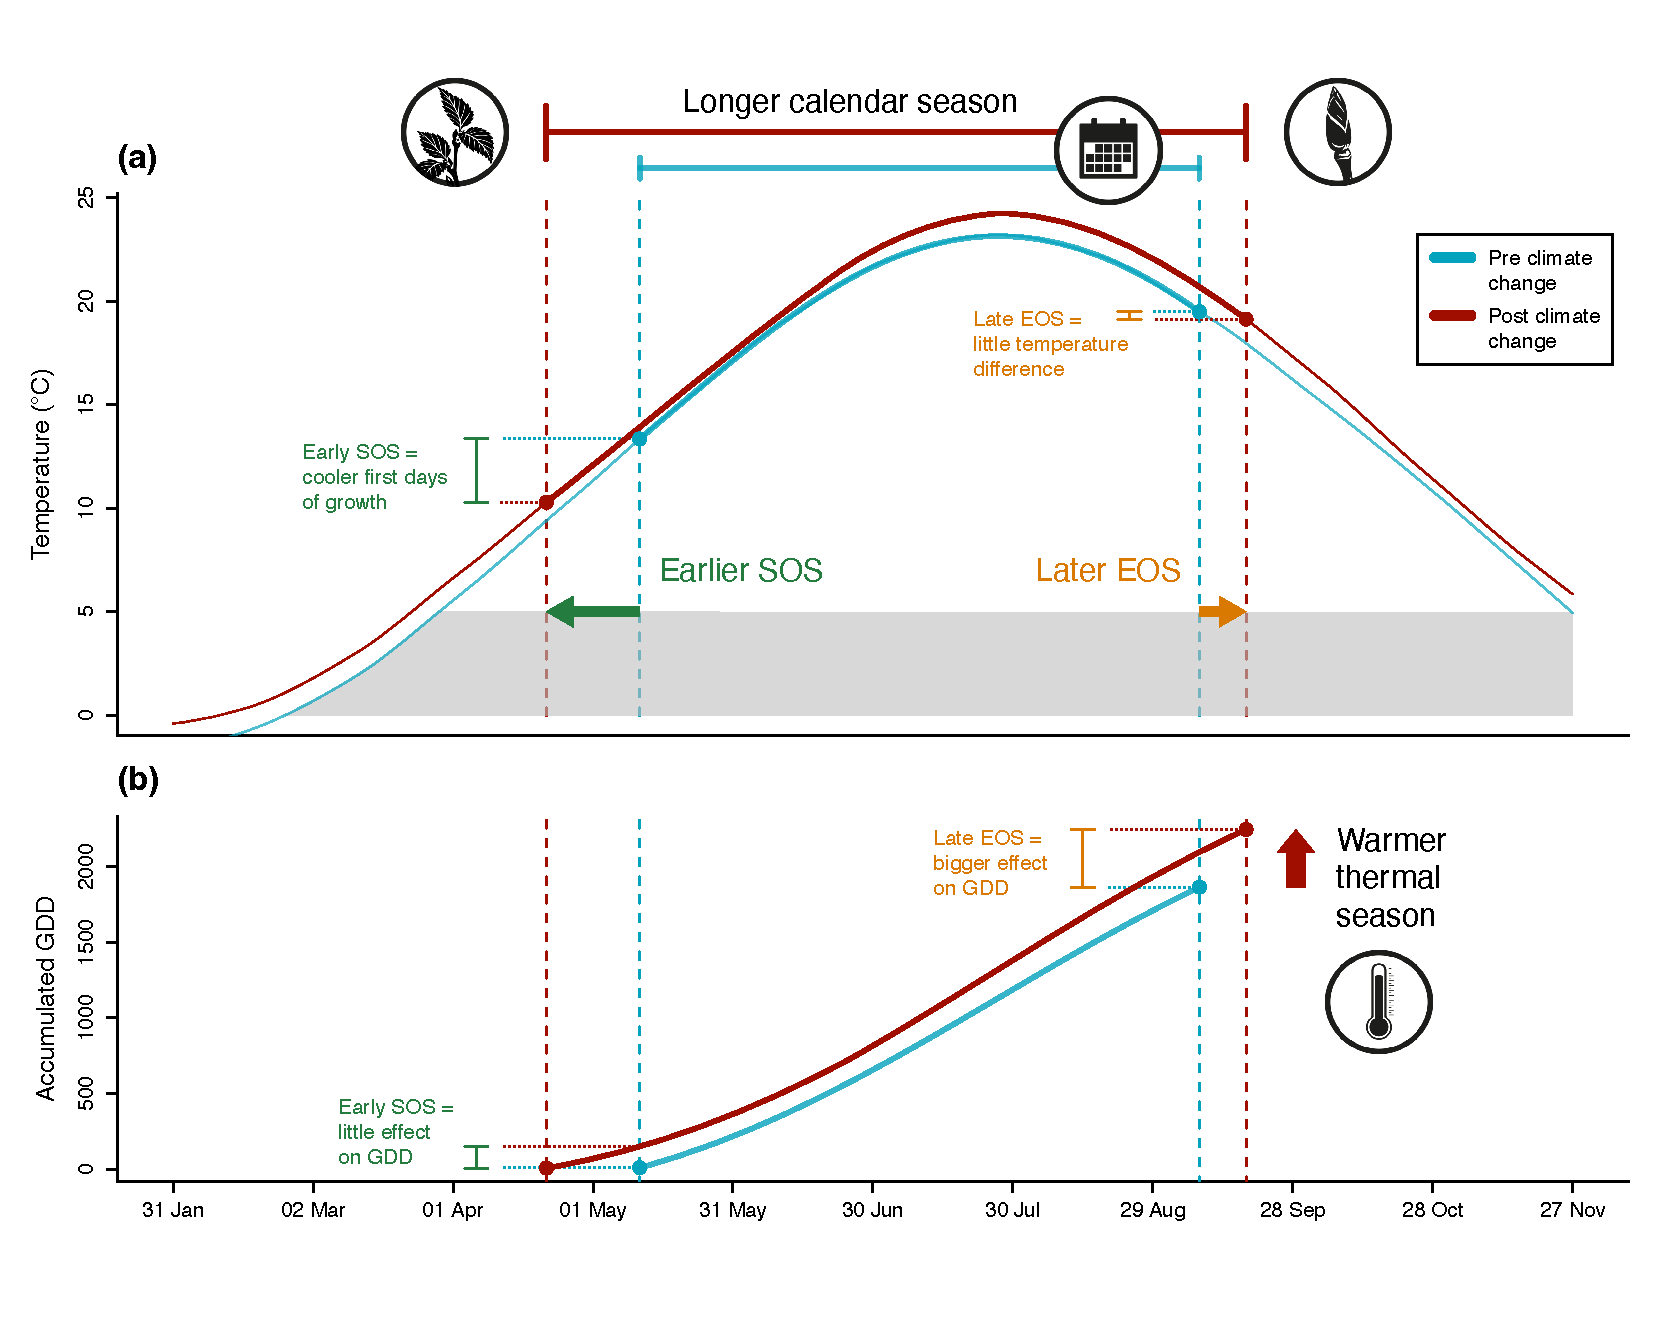
\includegraphics[width=0.9\textwidth]{../../analyses/figures/climate/gsconceptualfig_AdobeI.pdf}
\caption{Shifting growing season lengths with climate change affect both the temperature trees experience throughout the growing season (a), and how many growing degree days (GDD) they accumulate (b). With climate change, spring and autumn events have shifted, lengthening the calendar growing season. These longer seasons also changed the temperature trees experience early in their season, with cooler first days of growth (a) leading to little accumulation of GDD (b), and weaker shifts in days at the end of season (a) resulting in a higher GDD accumulation (b) due to warmer temperature during this period. Alongside these start and end of season shifts, warmer summer temperatures increased GDD accumulation, further warming their thermal seasons. The arrows represent hypothetical shifts in spring (green) and autumn (orange) phenology. We show changes in daily (smoothed) and accumulated temperatures before (1945-1965, in blue) and significant anthropogenic climate warming (2005-2025, in red), using mean daily temperature data from the Boston Logan International Airport Climate Station \citep{nationaloceanicandatmosphericadministration_local_2026}.}
\label{fig:GSfig}
\end{figure}

% <><><><><><><><><><><><><><><><><><><><><><><><><><><><><><><><><><><><><><><>
% METHODS
% <><><><><><><><><><><><><><><><><><><><><><><><><><><><><><><><><><><><><><><>
\clearpage
\section{Materials and Methods}

%-------------------------------------------------------------------------------
% Common garden setup
%-------------------------------------------------------------------------------
\subsection*{Common garden setup and data collection}
We collected seeds from 18 species of deciduous trees and shrubs from four provenances across a 3.5$^{\circ}$ latitudinal gradient (Figure \ref{fig:wcmuplotasite}a; Table \ref{tab:tab_species} and \ref{tab:climate}) in 2014-2015, germinated them following standard germination protocols and grew them to seedlings \citep{baskin_seeds_2014}. In the spring of 2017, we planted the seedlings outside at the Weld Hill Research Building at the Arnold Arboretum in Boston MA (42.30\degree N, 71.13\degree W). Plots were regularly weeded and watered throughout the duration of the study and were pruned in the autumn of 2020 \citep{buonaiuto_early_2026}. 

For the years 2018-2020, we monitored leaf phenology for all individuals in the common garden once or twice per week from February to December; the exact frequency varied within and across years (for more details, see Figure \ref{fig:phenoTimeSeries}). For this, we used a modified BBCH scale to observe two phenological stages: leafout which we defined as BBCH 15 and budset as BBCH 102 \citep[for more details, see:][]{finn_general_2007,buonaiuto_early_2026}. We had a total of 239 leafout and 230 budset observations (which we refer to as the `full datasets'), but for some individual trees in certain years we did not have data for both events; thus our total of matched full growing season duration (which we refer to as the `restricted dataset') is 227 observations.  

  In the spring of 2023, we collected tree ring samples from four species in the \textit{Betulaceae} family : grey alder (\textit{Alnus incana ssp. rugosa}), yellow birch (\textit{Betula alleghaniensis}), paper birch (\textit{Betula papyrifera}) and grey birch (\textit{Betula populifolia}). We collected cross-sections on 78 individuals by cutting the trunk above the root collar, and cores on 43 individuals using standard dendrochronological methods \citep{cook_methods_1990}, for a total of 81 individual trees (thus, we had three individuals with cores only; Table \ref{tab:tab_species}). We stored the cores in modified plastic straws to promote aeration and left them to dry with the cross-sections at ambient temperature for three months. 

% Wildchrokie provenances mu plot
\begin{figure}[!ht]
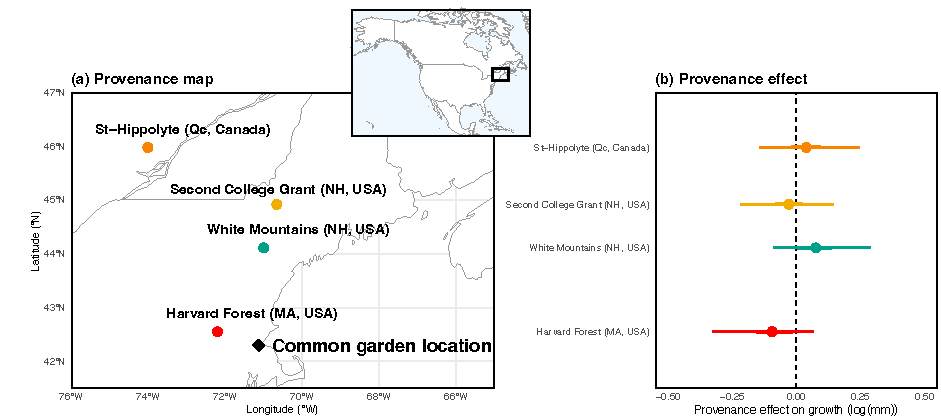
\includegraphics[width=1\textwidth]{../../analyses/figures/growthModelsMain/asiteMap_AI.pdf}
\caption{No effect of provenance on growth across a latitudinal gradient. Provenance where the seeds were sourced from is depicted as circles, while the diamond denotes the location of the common garden (a). The colors of the dots match the model estimates of (b), in which we show the ring width (log(mm); see Table \ref{tab:tab_GDD} for provenance parameter estimates) for each provenance with growing degree days as the predictor (effects were similar for the other predictors, see Tables \ref{tab:tab_GSL}, \ref{tab:tab_SOS}, \ref{tab:tab_EOS}). The dots represent the estimated mean of each provenance, with 50\% and 90\% uncertainty intervals (thicker and thinner lines, respectively; see also Figure \ref{fig:wcmuplotasitePerSpp} for a separate analyses, fitting the provenances per species)}
\label{fig:wcmuplotasite}
\end{figure}

%-------------------------------------------------------------------------------
% Sample processing, imaging and measuring
%-------------------------------------------------------------------------------
\subsection*{Sample processing, imaging and measuring}
We mounted cores on wooden mounts and sanded both the cores and cross-sections using progressively finer sandpaper grits (150, 300, 400, 600, 800, 1000), then scanned the cores and cross-sections at a resolution of 6250 dpi with a high-resolution tree ring scanner \citep{fong_tim_2026}. Using the digitized images, we measured ring widths with ImageJ \citep{schneider_nih_2012} at three standard locations for each cross-section (at {120\degree} from each other, averaging the three measurements to yield one ring width per year, per individual), and one ring width for each core. When we had cross-sections ($n = 78$) and cores ($n = 43$) for an individual, we used only the measurement from the cross-section ($n = 81 $). 

We performed visual cross dating. This consists of assigning a calendar year to each ring and comparing the year-to-year growth variation and anomalies across replicates of the same species \citep{stokes_introduction_1996}. We did not perform statistical crossdating or detrending because our chronologies (number of years of data) were extremely short \citep{radenPotentialIntraannualDensity2020a} and showed no evidence of consistent allometric trends (Figure \ref{fig:allom}). We controlled for effects of different years by including `year' in our models (see equation \ref{eq:mainMdl} in `Data analyses' below).

\subsection*{Data analyses}
To understand how growth shifted with season length, we used Bayesian hierarchical models, estimating how growth, measured as ring width, covaried with season length. We measured the season length in four different ways: GDD, GSL, SOS and EOS. Leaf phenology and growth are often closely synchronized in diffuse-porous species \citep[e.g., \textit{Betula;}][]{cufar_treering_2008} making leaf phenology a good proxy for setting the start and end of the growing season in these species \citep{marchand_timing_2021,silvestro_roots_2025,suzuki_phenological_1996}. Thus, we calculated the thermal season using growing degree days (GDD; mean daily temperature above 5\degree C) accumulated between leafout and budset, and the calendar season (or growing season length; GSL) as the number of days between leafout and budset. Finally, we used leafout for the start of season (SOS) and budset for the end of the season (EOS) as separate predictors that represent the boundaries of the growing season. For interpretability, we report ring width change in \% with the number of GDDs accumulated in an average week (seven days) in May (day of year 121 to 150 from 2018 to 2020), for the thermal season, and ring width change in \% per week of season length, leafout and budset for GSL, SOS and EOS, respectively. We report effects when the 90\% UI do not overlap with zero and consider a trend if the 50\% UI do not overlap with zero \citep{gelman_regression_2020}.

For daily climate data across all the years of phenological sampling (2018-2020), we combined two sources. For 2018 and 2019, we used data from the climate station located at Weld Hill research station \citep{arnoldarboretum_weather_2026}. Because the data were not available for that station after August 2020, we used data from the `Boston (Weld Hill)' weather station of the Network for Environment and Weather Applications (NEWA) for the whole year in 2020 \citep[see Figure \ref{fig:climOverlap} for the climate overlap between the two stations in 2020;][]{carroll_network_2026}. We used the North American Drought Monitor Maps to determine drought occurrence across years at our study location and used the proposed drought intensity index to qualify the presence of moderate, severe or extreme droughts \citep{nationalcentersforenvironmentalinformationncei_north_2026}. 

For each predictor, we estimated its effect on observed ring width ($\text{rw}$, with $i$ denoting each observation) for each tree ($treeid$) in each year ($year$) as:

\begin{equation}
\begin{aligned}
\log(\text{rw}_i) &\sim Normal(\mu_i, \sigma_y) \\ 
\mu_i &= \alpha + \alpha_{\text{species}} + \alpha_{\text{prov}} + \alpha_{\text{treeid}} + \alpha_{\text{year}} + \beta_{species} \times \text{season predictor[i]} \\
\alpha_{\text{prov}} &\sim Normal(0, \sigma_{\alpha \, \text{prov}}) \\
\alpha_{\text{treeid}} &\sim Normal(0, \sigma_{\alpha \, \text{treeid}}) \\
\end{aligned}
\label{eq:mainMdl}
\end{equation}

This model estimates a species-specific effect of each season length predictor (e.g. GDD) on growth ($\beta_{species}$), while also controlling for other variation due to species ($\alpha_{species}$), provenance ($\alpha_{prov}$), individual tree ($\alpha_{treeid}$) and year ($\alpha_{year}$). We ran the models using both natural units, and also using scaled predictors \citep[via $z$-scoring.][]{gelman_data_2006} to allow for direct comparison of effect sizes across different metrics.

We used weakly informative priors for all models (increasing the priors by 2$\times$ for the  models with all four predictors (GDD, GSL, SOS and EOS) did not qualitatively affect the results). We ran four chains with 2000 warm-up and 2000 sampling iterations each, for a total of 8000 sampling iterations and checked output diagnostics: chains had no divergent transitions, $\hat{R}$ values below 1.01, and effective sample sizes ($n_{\text{eff}}$) greater than 10\% of the model iterations. We also fit the models for SOS and EOS using both the restricted ($n =$ 227) and full datasets for each predictor (SOS $n =$ 239 and EOS $n =$ 230). We wrote our models using Stan \citep{carpenter_stan_2017} with the rstan package version 2.32.7 \citep{standevelopmentteam_rstan_2025} to run the Stan code in R \citep{rcoreteam_language_2021}.

In addition, we compared the relative effect of an extension in the SOS versus EOS using our estimated effect of GDD (Equation \ref{eq:mainMdl}). To do this, we averaged the GDD (mean daily GDD from 2005 to 2025) accumulated seven days before the median leafout (for SOS) and after the median budset (for EOS), for each species, across all years of our dataset. Then, with our estimated parameters, we report the \% effect of GDD on growth for an extended SOS and EOS: $\% \Delta \text{ring width} = (e^{\beta*GDD_{extSOS/EOS}}-1) \times 100$.

Because ring widths decrease with age---particularly with young trees \citep{fritts_dendroecology_1989}---we also ran the models using basal area increment (BAI) as the response variable. This allows for a more representative portrayal of annual growth increment by using the total ring area, instead of its width alone. To calculate BAI we summed each ring width separately at the three distinct locations on the cross sections yielding three radii from pith to bark. We then calculated the area of each ring by subtracting the radius from the inner ring from the outer ring: $\pi \times (\text{inner radius}^2 - \text{outer radius}^2)$, and averaged across the three BAI for each ring. 


% <><><><><><><><><><><><><><><><><><><><><><><><><><><><><><><><><><><><><><><>
% RESULTS
% <><><><><><><><><><><><><><><><><><><><><><><><><><><><><><><><><><><><><><><>
\section{Results}

%-------------------------------------------------------------------------------
\subsection*{Relationship between growth and thermal and calendar growing season}
%-------------------------------------------------------------------------------
Longer growing seasons increased growth for all species, but species differed in their response to the calendar season length versus accumulated GDD (thermal season). We report estimates as means and 90\% uncertainty intervals (UI) that correspond to ring width change in \% per one week unit (see `Data analyses' section in Methods for more details).
Warmer thermal seasons increased growth for paper birch (\textit{Betula papyrifera}; $\beta =$
15.96\% (UI: 6.05, 26.23)), grey birch (\textit{Betula populifolia}; $\beta =$
7.25\% (UI: 2.49, 12.35)), and yellow birch (\textit{Betula alleghaniensis}; $\beta =$
4.21\% (UI: 0.39, 8.07)). Grey alder (\textit{Alnus incana}) trended in the same direction ($\beta =$ 
2.25\% (UI: -1.10, 5.69)); Figure \ref{fig:wcmuplotbspp}a and e; Table\ref{tab:tab_GDD}).
Unlike its response to warmer thermal season, {\Ainc} grew more with longer calendar seasons ($\beta =$
5.25\% (UI: 0.33, 10.52)). {\Bpap} also grew more with longer calendar seasons ($\beta =$ 
20.69\% (UI: 5.38, 36.73)), while the other two \textit{Betula} did not, though they trended in the same way ({\Ball}: $\beta =$
3.41\% (UI: -2.56, 9.53), and {\Bpop}: $\beta =$
5.70\% (UI: -2.06, 13.76); Figure \ref{fig:wcmuplotbspp}b and f; Table \ref{tab:tab_GSL}). 
On a scaled axis \citep[through $z$-scoring,][]{gelman_data_2006}, the thermal and calendar season were similarly predictive (Figure \ref{fig:bsppZscored}). Results with basal area increment (BAI) for the GDD and GSL model were similar to ring width (see Table \ref{tab:BAItab} for GDD, and Table \ref{tab:BAItab_gsl} for GSL).

%-------------------------------------------------------------------------------
\subsection*{Growth at the start versus the end of the growing season}
%-------------------------------------------------------------------------------
Increased growth with longer seasons is often presumed to come from growth in the spring, since spring phenology has shifted much more than autumn phenology. Yet, only one species grew more with an earlier start of season, ({\Ainc} (one of the two species for which a longer calendar season increased growth: $\beta =$
-6.98\% (UI: -12.60, -1.10); more growth with an earlier start of season is represented as a negative slope; Figure \ref{fig:wcmuplotbspp}c and g; Table \ref{tab:tab_GSL} and \ref{tab:tab_SOS}). {\Bpop} trended in the opposite direction ($\beta =$
5.17\% (UI: -6.58, 17.74)), and {\Ball}, which did not grow more with a longer calendar season, grew less with an earlier start of season ($\beta =$
10.62\% (UI: 0.29, 21.43); Figure \ref{fig:wcmuplotbspp}c and g; Table \ref{tab:tab_SOS}). In contrast, we found most species grew more with a later end of season ({\Ball}: $\beta =$ 
12.33\% (UI: 5.25, 19.66), {\Bpop}: $\beta =$
10.07\% (UI: 2.28, 18.14), and {\Bpap}: $\beta =$
23.40\% (UI: 9.03, 38.98); Figure \ref{fig:wcmuplotbspp}d and h; Table \ref{tab:tab_EOS}), with the latter being the only one of those three that also grew more with longer calendar season. The estimates were unchanged when using the full (SOS: $n =$
239 and EOS: $n =$
230) or restricted datasets ($n =$ 
227; Figure \ref{fig:wcSOSEOScomparison}).

%-------------------------------------------------------------------------------
% Comparison between GSL and GDD at both start and end of season
%-------------------------------------------------------------------------------
More growth with a later EOS could be due to the warmer days at the end of the season. We found support for this from using our modeled estimates to predict how much growth would increase when extending the season at the start or end. We found that adding an estimated 7 days at the EOS increased growth across all species by 
10.65\% (UI: 6.05, 15.39), compared to an increase of
7.12\% (UI: 4.04, 10.27) from an earlier SOS (estimated using our model of GDD shown in Figure \ref{fig:wcmuplotbspp}, see `Data analyses' section in Methods for more details; Table \ref{tab:phenogain}). Differences in magnitude between an extension of SOS versus EOS were similar across species (Table \ref{tab:phenogain}).

%-------------------------------------------------------------------------------
\subsection*{Year and provenance level effects on growth}
%-------------------------------------------------------------------------------
We did not find any clear effect of year on growth, and there were no apparent differences in baseline growth between species (Figure \ref{fig:wcmuplotasite}b; Tables \ref{tab:tab_GDD}, \ref{tab:tab_GSL}, \ref{tab:tab_SOS}, \ref{tab:tab_EOS}). The limited variation between provenances ($\sigma = $
1.19 ring width (mm; UI:
1.02, 
1.61) was similar to variation across individual trees ($\sigma =$ 
1.18 ring width (mm; UI: 
1.04, 
1.31); Figure \ref{fig:wcmuplotatreeid}; Tables \ref{tab:tab_GDD}, \ref{tab:tab_GSL}, \ref{tab:tab_SOS}, \ref{tab:tab_EOS}).


% Figure mu across all species and climate predictors
\begin{figure}[!ht]
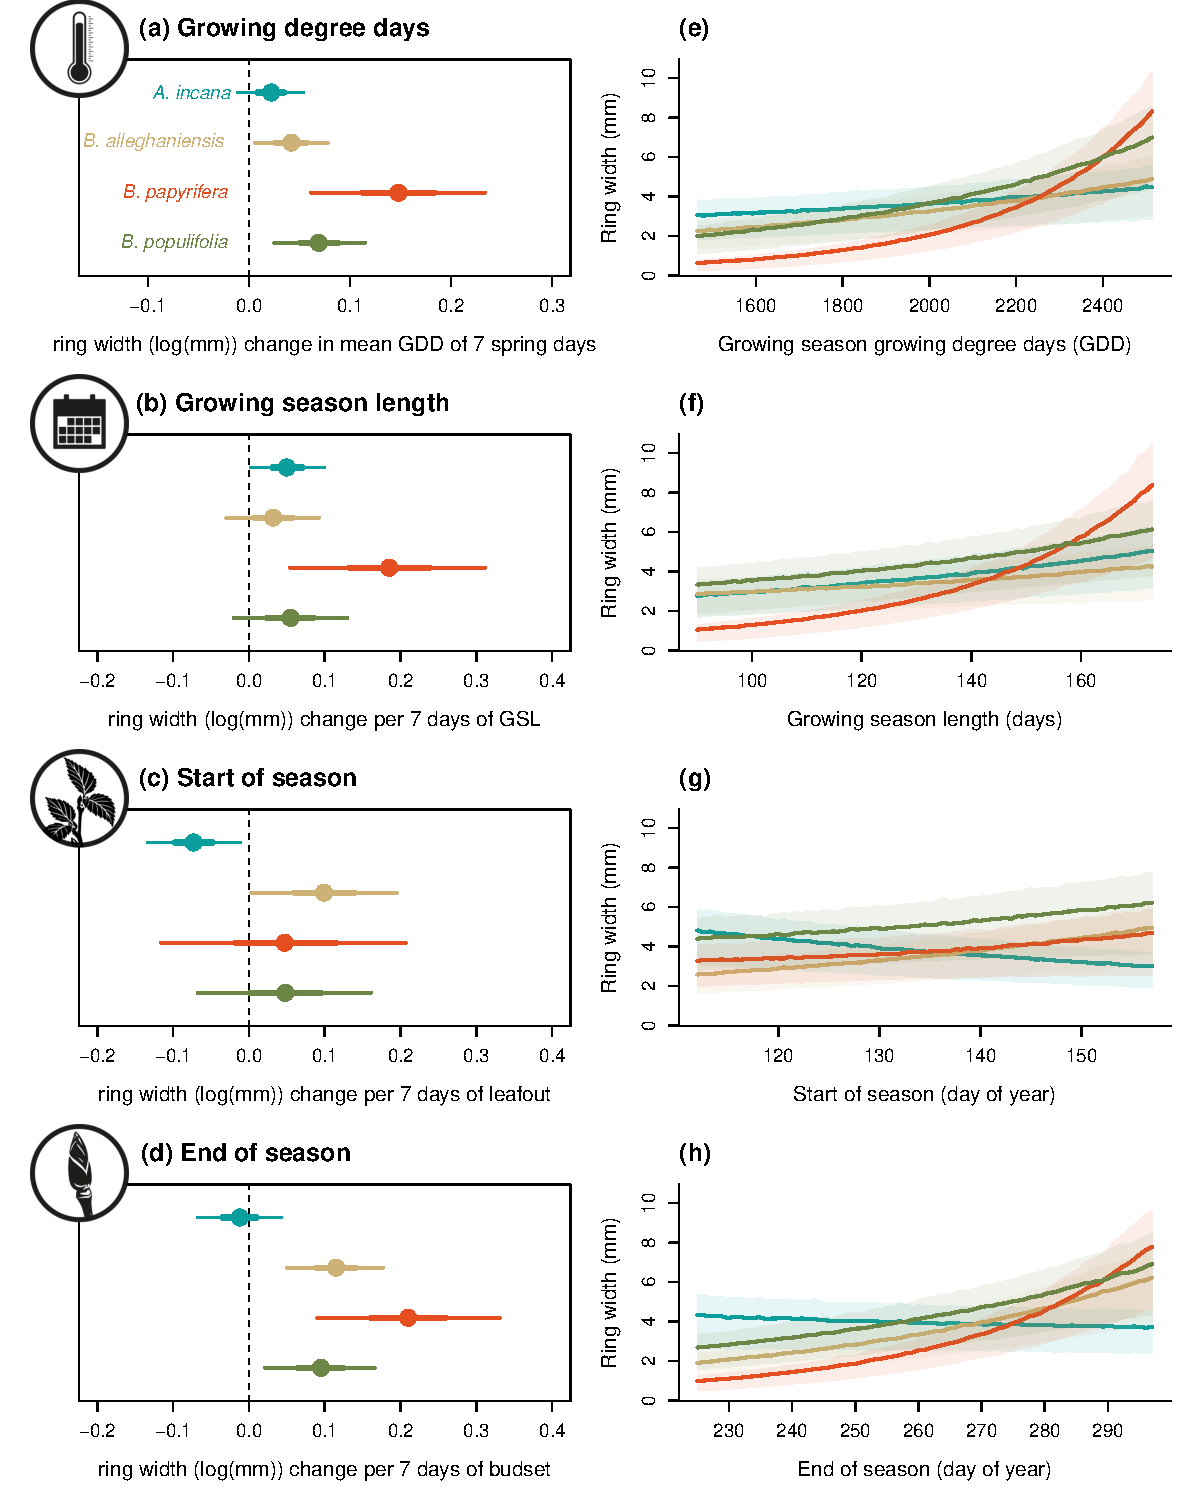
\includegraphics[width=0.8\textwidth]{../../analyses/figures/growthModelsMain/muALLbsppWlines.pdf}
\caption{Estimates of ring width change as a function of four different phenological predictors: growing degree days of the growing season (mean daily temperature above 5\degree C); growing season length, start of season, and end of season across four species: grey alder (\textit{Alnus incana}), yellow birch (\textit{Betula alleghaniensis}), paper birch (\textit{Betula papyrifera}) and grey birch (\textit{Betula populifolia}; species colors are the same across the panels). Panels on the left (a to d) represent the mean model slope estimates for each species (dots) with 50\% and 90\% uncertainty intervals (thicker and thinner lines, respectively), for each predictor, which we represent through ring width change in mm on the log scale per adjusted predictor (see `Data analyses' section in Methods for more details on predictor adjustment). Panels on the right (e to h) show the same estimated response of ring width (mm) as a function of each predictor, with the lines depicting the mean response at each predictor value, and the shaded area, the 50\% uncertainty intervals. See Tables \ref{tab:tab_GDD}, \ref{tab:tab_GSL}, \ref{tab:tab_SOS}, \ref{tab:tab_EOS} for parameter estimates, and Figures \ref{fig:wcxyGDD} and \ref{fig:wcxyGSL} for versions of these figures with empirical data.}
\label{fig:wcmuplotbspp}
\end{figure}

% <><><><><><><><><><><><><><><><><><><><><><><><><><><><><><><><><><><><><><><>
% DISCUSSION
% <><><><><><><><><><><><><><><><><><><><><><><><><><><><><><><><><><><><><><><>
\clearpage
\section{Discussion} 
We found that longer growing seasons increased growth for all four species, but the strength of this relationship varied depending on the metric used to measure season length. In particular, the thermal growing season was more often related to growth than the calendar season. Thus, our results support the hypothesis that the thermal season is a better predictor for growth \citep{chuine_processbased_2017,wang_simulation_1998}. They also suggest that the short and cool spring days early in the season contribute less to growth than additional days later in the season, when conditions are warmer \citep{buonaiuto_early_2026}. Further supporting this, we found a larger response of growth to the end of season than to its start, when considering each date separately \citep{zhang_drought_2021}.

Our finding that the end of season appears more related to growth than the start of season is aligned with increasing work suggesting that both season events together may dynamically determine growth \citep{zohner_effect_2023}. This implies that research focusing solely on the start of season \citep{dow_warm_2022,gaoEarlierStartThermal2022,wheeler_snow_2016} could miss when longer seasons lead to more growth. While studies have long called for more research on the end of season \citep{gallinat_autumn_2015,gunderson_forest_2012,piao_plant_2019,richardson_terrestrial_2012}, our results suggest we may especially need more work that monitors how growth and phenology shift across the season \citep{zani_increased_2020,zohner_effect_2023}. 

By accounting for differences in daily temperatures, the thermal season may align more closely to when and how fast plants can grow each day compared to the calendar season, which assumes a stable influence of each day on growth \citep{korner_four_2023}. Our results suggest significant growth occurs towards the end of the season, but would require data with a finer temporal scale (e.g., daily or weekly data through dendrometers and/or xylogenesis) to confirm this. To date, these studies showed strong species differences in when most growth happens during the season, though most studies are on mature trees \citep[e.g.][]{zweifel_are_2016,etzold_number_2022,balducci_stem_2019}. 

Our focus on juvenile trees may partly explain why we found increased growth with longer seasons \citep{augspurger_differences_2003,sweeneyComparisonTimingSpring2024}. Younger trees are generally more plastic than their adult forms \citep{augspurger_differences_2003,way_photoperiod_2015}, allowing them to take advantage of light early in the season or in response to forest gaps. If our juvenile trees grew in a mature forest, they would have been positioned below the canopy and exposed to stronger competition for light and other resources. Their growth response to longer seasons could therefore have been weaker than what we observed
\citep{cleland_effects_2024,augspurger_differences_2003,sweeneyComparisonTimingSpring2024,polgar_leafout_2011}. In addition, we grew our trees in a common garden with potentially more space between trees than in a natural setting (spacing was between 1.5 and 3 m), without any shade cloth. While other studies on mature trees have found the same response \citep{finziCarbonBudgetHarvard2020}, our results may have been more muted if the trees were grown in a forest setting. 

Understanding how juvenile trees respond to longer warmer season is critical for predicting how forests will regenerate and expand with the longer and warmer seasons of anthropogenic climate change. Plant phenology research has suggested that earlier seasons with warming favor species that shift earlier the most, with many studies that focused on invasive species appearing to support this \citep{wolkovich_temperaturedependent_2013,zettlemoyer_phenology_2019}. Yet, these studies are often on herbaceous species, and our results, along with other recent work \citep{zani_increased_2020,zohner_effect_2023}, suggest mid- and later-season effects may under-appreciate the performance implications in woody species in the absence of drought. Thus, more studies of how later season events correlate with invasions, and forest assembly more generally, could help understand how warming will impact forest regeneration and range expansion.

\subsection*{Species-level differences}
Our results suggest different growth strategies between species may yield different responses to longer seasons. Our most ruderal species, {\Ainc} was the only species to grow more with a longer calendar season and an earlier start of season. This suggests that species with more ruderal, flexible life history strategies may actually take advantage of growing more in the spring despite cooler, shorter days \citep{grime_evidence_1977,furlow_alnus_1997}. In contrast, growth of {\Bpap} and {\Bpop}, which are fast-growing but more conservative than {\Ainc}, was more driven by the end of season, suggesting that they may be able to exploit these late-season days characterized by warmer temperatures \citep{burns_silvics_1990}. Lastly, our slowest growing, longest-living species, {\Ball}, responded to both the start and end of season. This points towards a possible `neutralizing' response where an early start of season decreases growth, but a later end of season increases it, offsetting this species' response to a longer calendar season. 

Studies including an even wider span of growth strategies across species may find further differences. Our four study species all grow relatively fast, which should allow them to track changing conditions better than their slower-growing counterparts. While we found an overall positive trend of warmer seasons on growth, this might have changed if we used slower-growing, more conservative species \citep[such as \textit{Quercus};][]{burns_silvics_1990}. Current research suggests that leaf and wood phenology differ in their plasticity in response to changing environmental conditions across species and life stages \citep{dox_wood_2022}. Leaf phenology (e.g. leafout) in the spring is a highly plastic trait which varies substantially across years with different climates, tree age and also across species. Within a single community leafout can vary across species by over a month \citep{wolkovich_progress_2014}. How flexible growth is in response to changing growing season length and conditions thus appears to vary between species---and populations. 

Studies of large latitudinal gradients have found lower growth in trees sourced from poleward latitudes \citep{aitken_time_2016,soolanayakanahally_timing_2013}, yet we found little difference in growth across a latitudinal gradient of 3.5\degree. Thus, at least across this latitudinal range, local adaptation on growth appears weak. Supporting this, we found no evidence of a shifting end of season across provenances in these species, on average, despite decades of work finding that end of season events, such as budset, are usually more locally adapted than start of season events such as leafout \citep{kramer_effect_1936,habjorg_photoperiodic_1978,soolanayakanahally_timing_2013,aitken_time_2016,zeng_weak_2024}. In contrast to strong constraints on budset that should drive it to be timed similarly across years, a study of the same common garden including all tree and shrub species found that the end of season appeared to vary strongly by year and shift earlier with earlier start of season \citep{buonaiuto_early_2026}. Thus our results suggest that our current understanding of budset being strongly locally adapted, and thus varying little with temperature or the start of season, needs more study and at a wider geographical scale.

\subsection*{Implications for forest conservation and modeling}
Integrating our results into forest and larger-scale (e.g., land-surface) models requires considering how environmental conditions beyond temperature shift across the season, especially for soil moisture \citep{gaoEarlierStartThermal2022,li_widespread_2023}. While trees may have a longer period to grow, water availability may become insufficient to support continuous growth throughout the growing season \citep{lempereur_growth_2015, wang_seasonal_2025}. We regularly watered the trees in our common garden, likely relieving any major drought pressures, though studies beyond ours connected a later end of season and more growth \citep[see:][]{gaoEarlierStartThermal2022,wang_seasonal_2025}. In the range of our four species, drought occurrence has not yet increased \citep{nationalcentersforenvironmentalinformationncei_north_2026,agel_drought_2025}, suggesting that trees in the absence of water constraints may grow more with longer and warmer growing seasons \citep{cook_uncertainty_2011,agel_drought_2025,dorangeville_beneficial_2018}, as we found. The positive effect of a later end of season, however, could diminish if soil moisture becomes inadequate for growth \citep[as recently shown in our region by][]{jurado_increasing_2025}, and other temperate regions with decreased soil moisture have reported declines in tree growth \citep[e.g.,][]{spinoni_will_2018,zhang_drought_2021}, but we suggest our results here may be accurate for temperate northeastern North American forests.

The overall positive response we observed across multiple tree species to warmer seasons has important implications for carbon models, and related natural climate solutions. While juvenile trees store less carbon than their adult forms, they are crucial for forest regeneration and range expansion \citep[as discussed above, and see][]{luu_importance_2024}. In addition to their ecological role, juvenile trees generally predict adult tree responses qualitatively \citep{augspurger_differences_2003,wolkovich_why_2025}, despite certain ontogenic differences in stress residence and mortality rate across life stages \citep{caron_thermal_2021}. Thus our results on young trees can likely inform how their adult counterparts will respond to changing growing season conditions.

We also found that the start and end of season asymmetrically matter to growth, which means that how we model these phenological events in vegetation and related earth system models may be critical for accurate carbon dynamic predictions \citep{li_comparison_2022}. Such models usually assume a temperature-sensitive start of season and a photoperiod-controlled, and thus less variable, end of season \citep{chen_comparison_2022,melaas_multiscale_2016}. This results in a disproportionate influence of the start compared to the end of season on tree growth, unlike what our results suggest. Such a representation of what drives the temporal boundaries of the growing season may feed into oversimplified explanations of the processes regulating tree growth with future climate change. 

\section*{Acknowledgements}
We thank to Sally Aitken and reviewers for comments that helped improved the manuscript and Charlotte Capistran-Champoux for her help with figure design and visual improvements. This work was supported by NSERC Canada Graduate Research Scholarship – Master’s (CGS-M) to C.R-D. and NSERC Discovery to E.M.W. The text of this article was written without any GenAi, nor was it used for any creative or idea generation process. C.R-D used Claude Sonnet 5 (and prior versions) for performing simple repetitive coding tasks, including help with the figure coding, data cleaning and improving coding workflow efficiency. All other co-authors did not use GenAi for their contribution to the paper.

\section*{Author contribution}
E.M.W. proposed the original research idea. C.R-D. conducted the analyses with V.V.d.M. and E.M.W. help throughout. D.M.B, C.C collected the phenology data and C.R-D processed the tree ring samples that were collected by N.P., D.M.B, D.L. and E.M.W. C.R-D and E.M.W. wrote the initial draft and all authors reviewed and approved the manuscript.

\section*{Data availability statement}
We will publish the data on KNB at the time of publication.

%<><><><><><><><><><><><><><><><><><><><><><><><><><><><><><><><><><><><><><><><>
% REFERENCES %
%<><><><><><><><><><><><><><><><><><><><><><><><><><><><><><><><><><><><><><><><>
\bibliography{ExportedItems}
\bibliographystyle{besjournals} 

\end{document}
